\part{Examples}

\section{Math}

Consider the formula
$$p = (1-\lambda)\cdot\lambda$$
but ignore it.

\section{Images}
Types can be inferred by a proof-like system with the following core rules:
\begin{center}
 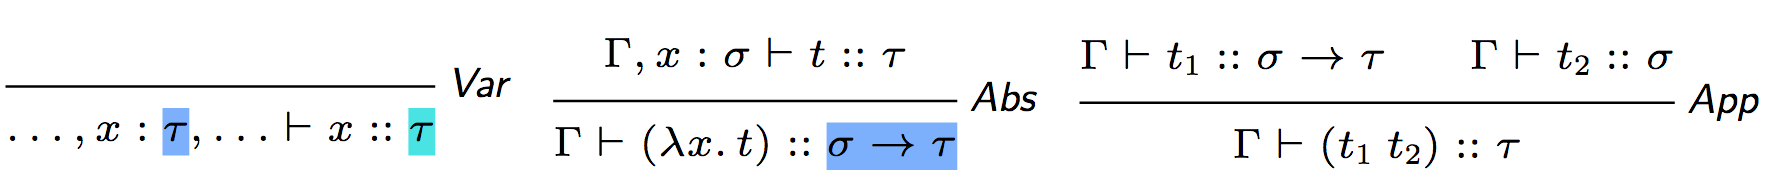
\includegraphics[scale=0.21]{type_inference}
\end{center}

\section{Lists}
\begin{enumerate}[a)]
	\item \textbf{Base Types}: Double, ...
	\item \textbf{Compound Types:} Lists, Tuples, ...
	\item \textbf{Type Classes}, have Instances, offer restricted form of polymorphism. Similar to Interfaces. E.g the type class \verb+Eq+ represents a set of Types.
	\item \textbf{Algebraic Types}, similar to structs.
		\begin{itemize}
			\item Enumeration Types
			\item Product Types
		\end{itemize}
\end{enumerate}

\section{Code}
Multiline Code Example:
\begin{lstlisting}
primes = sieve [2 ..]
sieve xs = head xs : sieve (dropMults (head xs) 
                           (tail xs))
\end{lstlisting}

Code can be placed in line, e.g. \verb+data Tree = Leaf Int | Node Tree Tree+ with Verbatim.

\section{Theorems and Co.}

\Def[Probability Space] \\
blabla \\

\Theorem[Total Probability \& Bayes' Rule] \\
blabla \\

\Lemma[Independance] \\
blabla

\section{Boxes}

\begin{boxred}
\textbf{Neyman-Pearson-Lemma:} \\ Let 
$\Theta_{0}=\left\{\vartheta_{0}\right\}$ and $\Theta_{A}=\left\{\vartheta_{A}\right\}$. Further let \\
$T:=R\left(X_{1}, \ldots, X_{n} ; \vartheta_{0}, \vartheta_{A}\right)$ and $K:=(c, \infty)$ as well as $\alpha^{*}:=P_{\vartheta_{0}}[T \in K]=P_{\vartheta_{0}}[T>c]$.

$\implies$ The Likelyhood-Ratio-Test with statistic $T$ and rejection region $K$ is \textit{optimal} in the sense that: Every other test with significance level $\alpha \leq \alpha^{*}$ has a smaller power, i.e. a larger probability of type II error.
\end{boxred}


In general the hypothesises are not \textit{simple}. The following quotient is usually a sensible test statistic in these cases:
\begin{boxemerald}
The generalized Likelyhood-Ratio is given by
$$
R\left(x_{1}, \ldots, x_{n} ;\right):=\frac{\sup_{\vartheta \in \Theta_A} L\left(x_{1}, \ldots, x_{n} ; \vartheta\right)}{\sup_{\vartheta \in \Theta_0} L\left(x_{1}, \ldots, x_{n} ; \vartheta\right)}
$$
\end{boxemerald}


\begin{boxyellow}
\textbf{z-Test, i.e. normal with known variance:} 	

	Assume $X_{1}, \ldots, X_{n}$ i.i.d. $\sim \mathcal{N}\left(\vartheta, \sigma^{2}\right)$
	\begin{enumerate}[a)]
		\item \textit{Statistic Under $H_0$}:
		\[
			T=\frac{\overline{X_n}-\mu_0}{\sigma/\sqrt{n}} \sim \mathcal{N}(0,1)
		\]
		\item \textit{Rejection Region}:
		\begin{itemize}
			\item $\vartheta_A>\vartheta_{0}$: $K = \left[z_{1-\alpha},\infty\right)$
			\item $\vartheta_A<\vartheta_{0}$: $K = \left(-\infty, z_\alpha\right]$
			\item $\vartheta_A\neq\vartheta_{0}$: $K = (-\infty, z_{\frac{\alpha}{2}}]\cup [z_{1-\frac{\alpha}{2}},\infty)$
		\end{itemize}
	\end{enumerate}	
where $\Phi^{-1}(\alpha)=z_\alpha$ and for convenience $z_{0.95}=1.645$, $z_{0.975}=1.960$.
\end{boxyellow}

\begin{boxlavender}
The generalized Likelyhood-Ratio is given by
$$
R\left(x_{1}, \ldots, x_{n} ;\right):=\frac{\sup_{\vartheta \in \Theta_A} L\left(x_{1}, \ldots, x_{n} ; \vartheta\right)}{\sup_{\vartheta \in \Theta_0} L\left(x_{1}, \ldots, x_{n} ; \vartheta\right)}
$$
\end{boxlavender}

